%%%%%%%%%%%%%%%%%%%%%%%%%%%%%%%%%%%%%%%%%%%%%%%%%%%%%%%%%%%%%%%%%%%%%%
% This layout was adapted from one found at latextemplates.com which
% was adapted from another.
%
% License: CC BY-NC-SA 3.0
% (http://creativecommons.org/licenses/by-nc-sa/3.0/)
%
% Original header:
%
% This is a LaTeX version of the sample laboratory report from
% Virginia Tech's copyrighted 08-09 CHEM 1045/1046 lab manual.
% Reproduction of this one appendix section for academic purposes
% should fall under fair use.
%
%%%%%%%%%%%%%%%%%%%%%%%%%%%%%%%%%%%%%%%%%%%%%%%%%%%%%%%%%%%%%%%%%%%%%%

\documentclass{article}

\usepackage{graphicx} % Lets us use images
\usepackage[acronym]{glossaries} % Lets us use acronyms

\author{Charles Pittman}
\title{ELEC-311\\ Project 1\\ Combinational Circuit Design}
\date{October 1, 2013}

\loadglsentries{acronyms} % Actually loads 'acronyms.tex'
\makeglossaries

\begin{document}

\maketitle % Inserts title, author, and date from above

\pagebreak

% Removes indentation from paragraphs: \setlength\parindent{0pt}

% Number the enumerate environment (unordered lists) by letter:
\renewcommand{\labelenumi}{\alph{enumi}.}

\section{Objective}
\label{sec:objective}

% Multiple objectives:
 \begin{description}
 \item[First Objective] \hfill \\
   Given a function, design a combinational logic logic circuit.
 \item[Second Objective] \hfill \\
   Minimize the circuit using a Karnaugh map.
 \item[Third Objective] \hfill \\
   Create the circuit using only NAND gates.
 \end{description}

\section{Discussion}
\label{sec:procedure}

The circuit being studied is shown in Figure~\ref{fig:circuit}.
Working from right to left, the Boolean equation for the circuit can
be written: $(\overline{S} \cdot I_0 + I_1) \cdot E \cdot (I_0 + S
\cdot I_1)$.  A truth table for this equation is shown below.

After sketching the circuit with the Xilinx schematic capture, the
logic was translated to run on a Basys2 (\gls{fpga} board used).
Switches on the board were used to input a string of bits, with an LED
showing the function's result.

% \begin{figure}[hbtp]
%   \centering
%   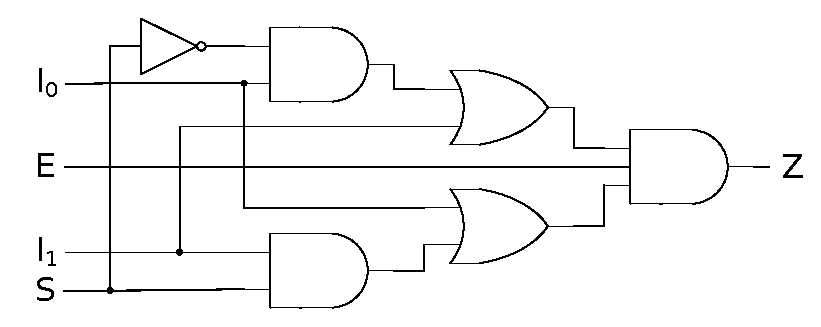
\includegraphics[width=\textwidth]{img/circuit}
%   \caption{Circuit to be analyzed.}
%   \label{fig:circuit}
% \end{figure}

\begin{table}[hbtp]
  \label{tab:truth}
  \centering
  % This LaTeX table template is generated by emacs 24.3.1
  \begin{tabular}{cccc|c}
    P1 & P0 & Q1 & Q0 & GT \\
    \hline
    0 & 0 & 0 & 0 & 0 \\
    0 & 0 & 0 & 1 & 0 \\
    0 & 0 & 1 & 0 & 0 \\
    0 & 0 & 1 & 1 & 0 \\
    0 & 1 & 0 & 0 & 1 \\
    0 & 1 & 0 & 1 & 0 \\
    0 & 1 & 1 & 0 & 0 \\
    0 & 1 & 1 & 1 & 0 \\
    1 & 0 & 0 & 0 & 1 \\
    1 & 0 & 0 & 1 & 1 \\
    1 & 0 & 1 & 0 & 0 \\
    1 & 0 & 1 & 1 & 0 \\
    1 & 1 & 0 & 0 & 1 \\
    1 & 1 & 0 & 1 & 1 \\
    1 & 1 & 1 & 0 & 1 \\
    1 & 1 & 1 & 1 & 0 \\
  \end{tabular}
  \caption{Truth table for circuit in Figure~\ref{fig:circuit}}
\end{table}

\section{Results}
\label{sec:results}
To verify the \gls{fpga}'s configuration, each entry from the truth
table was input and the output confirmed to match the expected value.
As an additional exercise, the circuit was simplified with Boolean
algebra, and tested as above.  The simplified circuit is shown in
Figure~\ref{fig:circuit_simp}.  The truth table, shown below, is
identical since the two circuits are equivalent.

% \begin{figure}[hbtp]
%   \centering
%   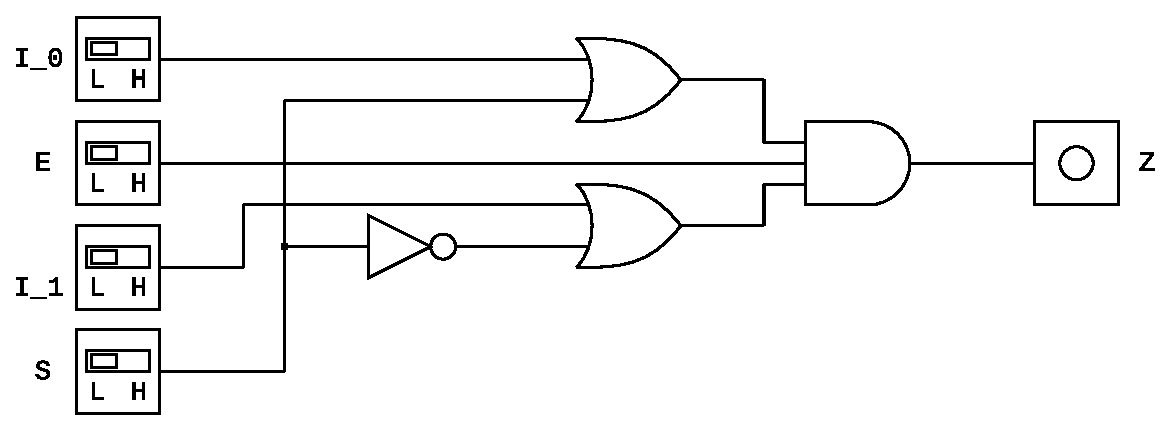
\includegraphics[width=\textwidth]{img/circuit_simp}
%   \caption{Simplified version of the circuit in Figure~\ref{fig:circuit}}
%   \label{fig:circuit_simp}
% \end{figure}

\begin{table}[hbtp]
  \label{tab:truth_simp}
  \centering
  % This LaTeX table template is generated by emacs 24.3.1
  \begin{tabular}{cccc|c || cccc|c}
    $I_0$ & $E$ & $I_1$ & $S$ & $Z$ & $I_0$ & $E$ & $I_1$ & $S$ & $Z$ \\
    \hline
    0 & 0 & 0 & 0 & 0 & 1 & 0 & 0 & 0 & 0 \\
    0 & 0 & 0 & 1 & 0 & 1 & 0 & 0 & 1 & 0 \\
    0 & 0 & 1 & 0 & 0 & 1 & 0 & 1 & 0 & 0 \\
    0 & 0 & 1 & 1 & 0 & 1 & 0 & 1 & 1 & 0 \\
    0 & 1 & 0 & 0 & 0 & 1 & 1 & 0 & 0 & 1 \\
    0 & 1 & 0 & 1 & 0 & 1 & 1 & 0 & 1 & 0 \\
    0 & 1 & 1 & 0 & 0 & 1 & 1 & 1 & 0 & 1 \\
    0 & 1 & 1 & 1 & 1 & 1 & 1 & 1 & 1 & 1 \\
  \end{tabular}
  \caption{Truth table for circuit in Figure~\ref{fig:circuit_simp}}
\end{table}

\end{document}
